%%%%%%%%%%%%%%%%%%%%%%%%%%%%%%%%%%%%%%%%%%%%%%%%%%%%%%%%%%%%%%%%%%%%%%%%%%%%%%%%%%%%%%%%%%%%%%%%%%%%%%%%%%%%%%%%%%%%%
\section{Objetivo}
El objetivo de este proyecto es automatizar una fábrica de pastillas de complementos alimenticios.

En este documento se especificarán los procesos necesarios para tal fin, las condiciones que deben cumplir los mismos, así como los planos para el correcto posicionamiento de las máquinas y el presupuesto con el coste aproximado del proyecto. 
 
%%%%%%%%%%%%%%%%%%%%%%%%%%%%%%%%%%%%%%%%%%%%%%%%%%%%%%%%%%%%%%%%%%%%%%%%%%%%%%%%%%%%%%%%%%%%%%%%%%%%%%%%%%%%%%%%%%%%%
\section{Ubicacion}

La fábrica se encuentra en Calle de la Fundición 8, Rivas-Vaciamadrid, Madrid, España.

%%%%%%%%%%%%%%%%%%%%%%%%%%%%%%%%%%%%%%%%%%%%%%%%%%%%%%%%%%%%%%%%%%%%%%%%%%%%%%%%%%%%%%%%%%%%%%%%%%%%%%%%%%%%%%%%%%%%%
\section{Antecedentes}
La propiedad ha adquirido la nave industrial tras la quiebra de un supermecado y ha contactado con esta ingeniería para realizar un proyecto de instalación de una fábrica de comprimidos. 

La nave mide ????????? metros de largo por ????????? metros de ancho, con una superficie útil de ????????? metros cuadrados.  
Incluye asimismo un espacio de oficina de dos niveles.  

Todo el recinto está dotado de los sistemas de ventilación y seguridad requeridos por la legislación vigente.

%%%%%%%%%%%%%%%%%%%%%%%%%%%%%%%%%%%%%%%%%%%%%%%%%%%%%%%%%%%%%%%%%%%%%%%%%%%%%%%%%%%%%%%%%%%%%%%%%%%%%%%%%%%%%%%%%%%%%
\section{Normativa}

\subsection{REBT}

Se sigue el Reglamento Electrotécnico de Baja Tensión

\subsection{Código Técnico de la Edificación}

\subsection{Normativas relativas a complementos alimentarios}

\subsection{Normativas de seguridad y salud}


%%%%%%%%%%%%%%%%%%%%%%%%%%%%%%%%%%%%%%%%%%%%%%%%%%%%%%%%%%%%%%%%%%%%%%%%%%%%%%%%%%%%%%%%%%%%%%%%%%%%%%%%%%%%%%%%%%%%%
\section{Descripción general}
 
\subsection{Planta}
El recinto tiene una superficie de ??????????? metros cuadrados, incluyendo la nave con las oficinas y un espacio de maniobra para camiones.
La nave tiene una superficie útil de ????????? metros cuadrados y se divide en tres zonas distintas: zona de carga y descarga de materiales, zona de almacenamiento de materia prima, zona de almacenamiento del produto finalizado y zona de máquinas donde se realiza el proceso de fabricación.
\\

Los camiones entran por en el recinto y tras maniobrar en el espacio habilitado para ello entran marcha atrás en la nave, donde los empleados procederán a descargarlo con la ayuda de toros mecánicos. Los sacos con la materia prima en polvo, así como los cartones para ensamblar las cajas, se almacenan en estanterías de palés situados delante del inicio del proceso. 
\\

En la zona de máquinas se lleva a cabo todo el proceso de transformación del polvo a cajas de pastillas. Contiene un horno de polvo, una máquina de compresión, una máquina de pruebas, un tambor de revestimiento, una máquina de formación de blisters y una última de embalaje, así como cintas para transportar los distintos elementos y dos brazos robóticos para colocar el producto final. El producto final se almacena en palés en estanterías cerca de la puerta para agilizar el proceso de carga del camión y por tanto perder menos tiempo.
\\

El espacio de oficinas cosiste de una recepción y un centro de control en la planta baja y un despacho y puestos de trabajo en el segundo nivel. Ambos pisos disponen de baños.

\subsection{Procesos}
Cuando el horno emita una señal de aviso un operario procederá a llenar el depósito de dicho horno con la materia prima. Una vez lleno, el horno libera el polvo uniformemente sobre una cinta transportadora. Esta lo transporta por el horno de manera ondulante para eliminar cualquier tipo de humedad. 
\\

A la salida del horno el polvo es introducido en una máquina de compresión, donde es convertido en pastillas y se le imprime el nombre de la pastilla.  Acto seguido pasa por una máquina de comprobación, que desecha cualquier pastilla que haya resultado demasiado frágil por seguir húmeda tras el horno. Las pastillas desechadas, se trituran y depositan en un recipiente para que el operario lo reintroduzca en el horno en la siguiente iteración. 
\\

El resto de pastillas continúa hasta un tambor donde se les da un revestimiento de agua con colorantes para su identificación y conservación, al endurecer así la capa exterior y evitar que se deshagan. Tras ser rociadas por pulsos muy rápidos y cortos para favorecer un secado rápido son transportadas a una máquina de sellado.
\\

En esta máquina se dejan caer pastillas hasta llenar un depósito, donde mediante un sensor indica el llenado. La selladora coloca las pastillas en posición segun la matriz utilizada. Paralelamente tira del rollo de plástico en lámina y lo coloca debajo de la parte superior. Al bajar, ésta deforma la lámina con unos cabezales calientes y crea los habitáculos donde inmediatamente inserta las tabletas. Acto seguido se corta el plástico y este avanza a la siguiente posición donde se le coloca una lámina de alumnio con el logo impreso y es sellado por calor al bajar la parte superior en la siguiente iteración. 
\\

Finalmente se transportan los blisters sellados por otra cinta transportadora a la máquina de empaquetado, que coge las cartulinas de las cajas y las dobla para darles su forma final e inserta los blisters en la caja, asi como un folleto explicativo previamente impreso y doblado. Las cajas con el produto final se dejan caer por una rampa hasta una mesa donde un brazo robótico equipado con una cámara coge las cajas individuales y las coloca en cajas de lotes en un palé para ser recogido por un operario y almacenado en una estantería. Un segundo brazo robótico coje un palé de una pila de palés vacíos y lo coloca en la posición del anterior.
\\




%%%%%%%%%%%%%%%%%%%%%%%%%%%%%%%%%%%%%%%%%%%%%%%%%%%%%%%%%%%%%%%%%%%%%%%%%%%%%%%%%%%%%%%%%%%%%%%%%%%%%%%%%%%%%%%%%%%%% 
\section{Elementos del sistema}

\subsection{Instalación eléctrica}
\subsection{Maquinaria}
	\subsubsection{Máquina de secado de polvo}
	\subsubsection{Máquina de compresión en tabletas}
	\subsubsection{Máquina de verificación de dureza de tabletas}
	\subsubsection{Máquina de revestimiento de tabletas}
	\subsubsection{Máquina de sellado de blisters }
	\subsubsection{Máquina de fabricación de cajas}	
	\subsubsection{Máquina de empaquetado}
	\subsubsection{Robot de paletizado}
%%%%%%%%%%%%%%%%%%%%%%%%%%%%%%%%%%%%%%%%%%%%%%%%%%%%%%%%%%%%%%%%%%%%%%%%%%%%%%%%%%%%%%%%%%%%%%%%%%%%%%%%%%%%%%%%%%%%%	
\section{Sistema propuesto}
%%%%%%%%%%%%%%%%%%%%%%%%%%%%%%%%%%%%%%%%%%%%%%%%%%%%%%%%%%%%%%%%%%%%%%%%%%%%%%%%%%%%%%%%%%%%%%%%%%%%%%%%%%%%%%%%%%%%%
\section{Anexos}

   
\subsection{Anexo de cálculos:}

\subsubsection{Cálculos de la Instalación eléctrica}
\paragraph{Diseño del cuadro general de protección y mando}
\paragraph{Cálculo de las líneas de alimentación de cada máquina}
\paragraph{Cálculo de las líneas para las tomas de corriente de uso general}
\paragraph{Cálculo de las líneas para las tomas de corriente con SAI}
\paragraph{Cálculo de las líneas para iluminación}
\paragraph{Cálculo de las líneas para iluminación de emergencia}

\subsubsection{Cálculo de las instalaciones de automatización}
\paragraph{Sensores }
\paragraph{Cuadro centralización de automatización}
\paragraph{Rack con PC industrial conectado a la red de la fábrica}
\subsubsection{Instalaciones de seguridad}
\paragraph{Protección de las personas}
\paragraph{Protección contra intrusión}

\subsection{Anexo de código}
\newpage
\subsection{Anexo de catálogos}
\subsubsection{Máquina de secado de polvo}
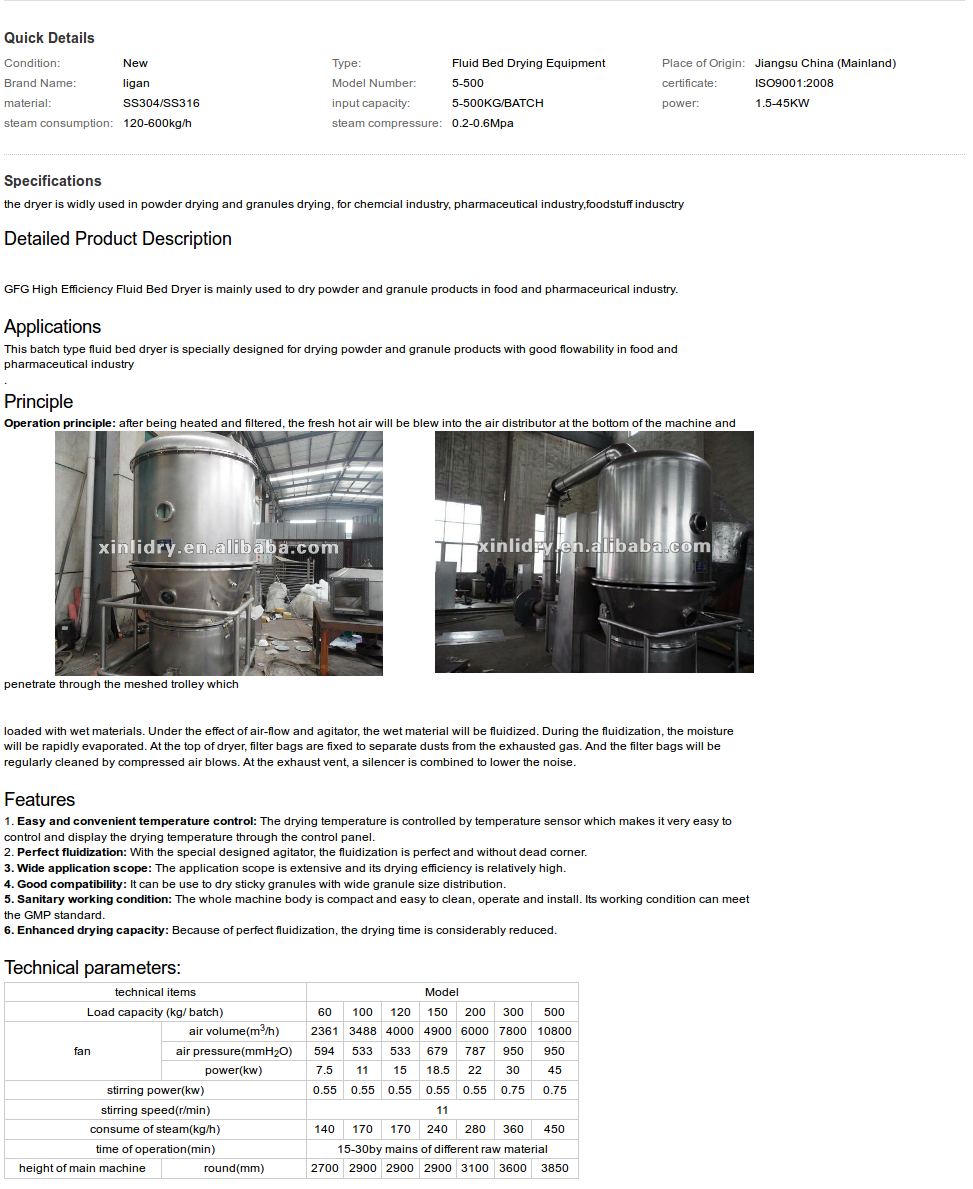
\includegraphics[width=15cm,height=20cm,keepaspectratio]{Datasheets/1MaquinaSecado.png} 
\newpage

\subsubsection{Máquina de compresión en tabletas}
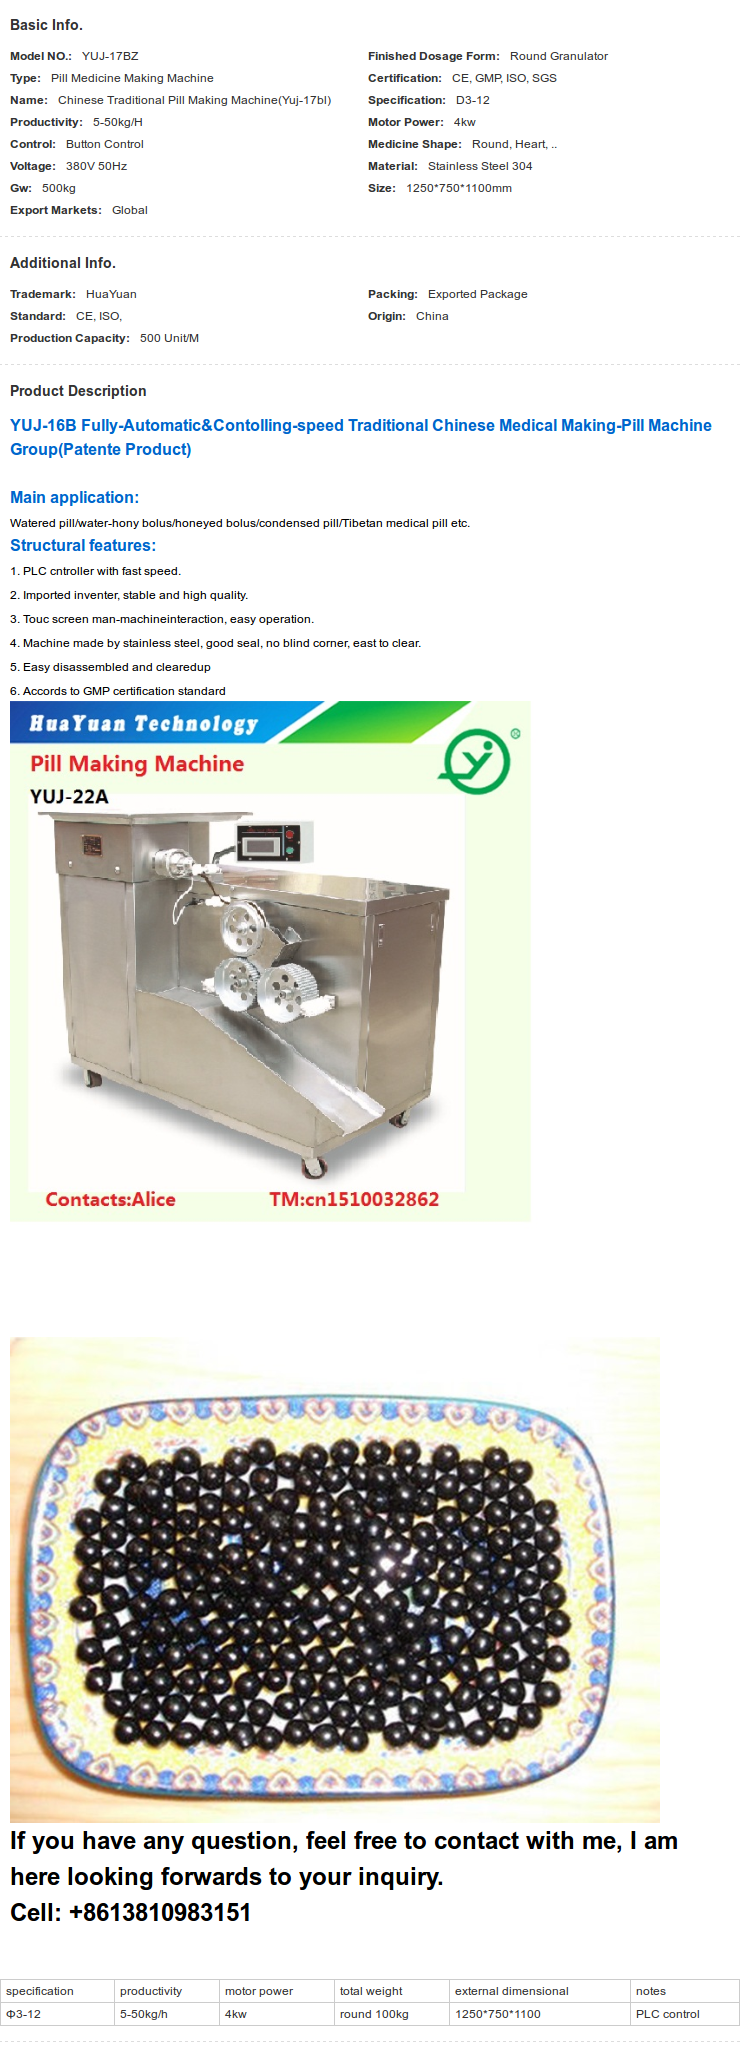
\includegraphics[width=15cm,height=20cm,keepaspectratio]{Datasheets/2MaquinaPrensado.png} 
\newpage

\subsubsection{Máquina de verificación de dureza de tabletas}
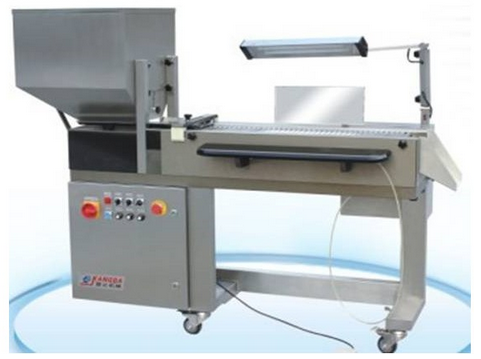
\includegraphics[width=5cm,height=4cm,keepaspectratio]{Datasheets/3Foto.png} 
\\
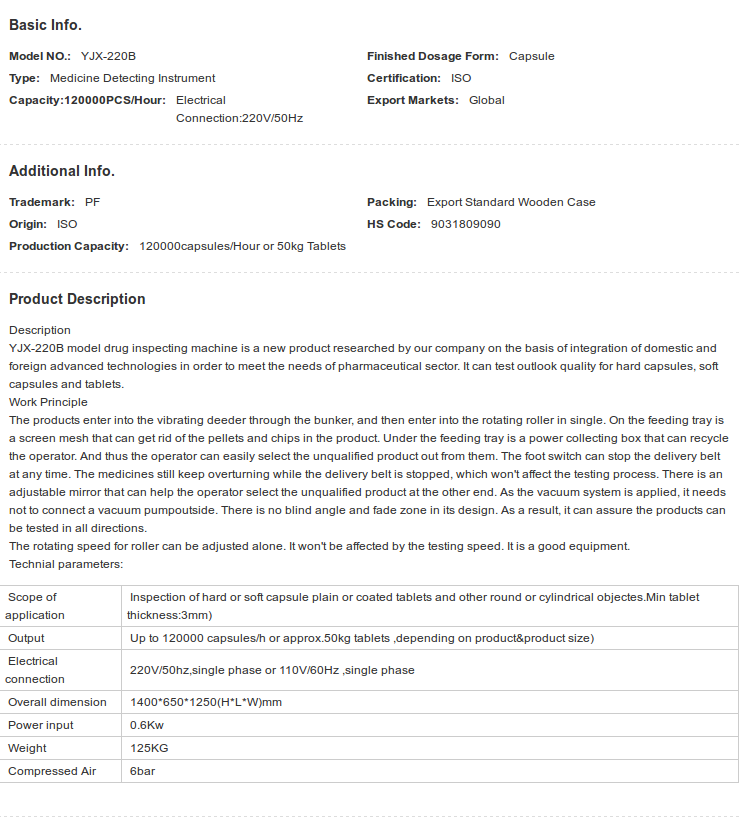
\includegraphics[width=15cm,height=20cm,keepaspectratio]{Datasheets/3MaquinaVerificacion.png} 
\newpage

\subsubsection{Máquina de revestimento de tabletas}
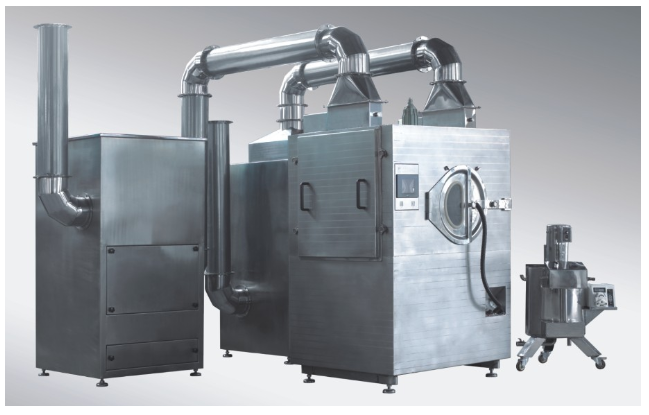
\includegraphics[width=5cm,height=4cm,keepaspectratio]{Datasheets/4Foto.png} 
\\
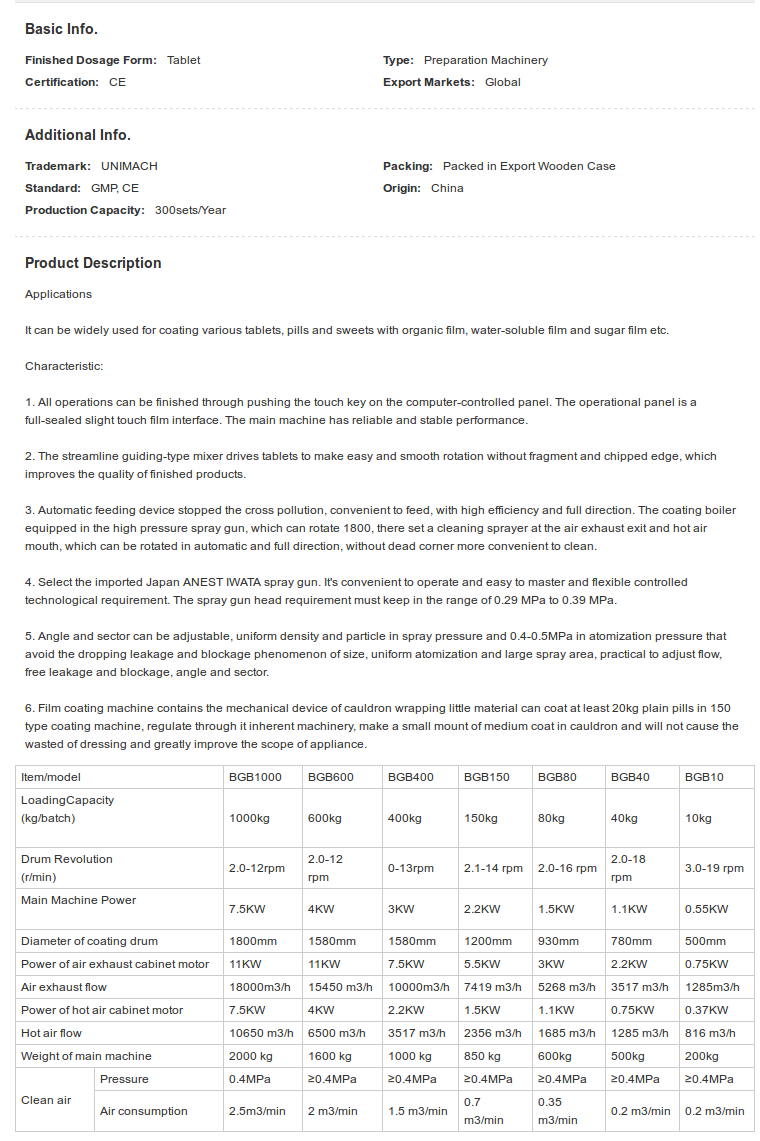
\includegraphics[width=15cm,height=20cm,keepaspectratio]{Datasheets/4MaquinaRevestimiento.png} 
\newpage

\subsubsection{Máquina de sellado de blisters}
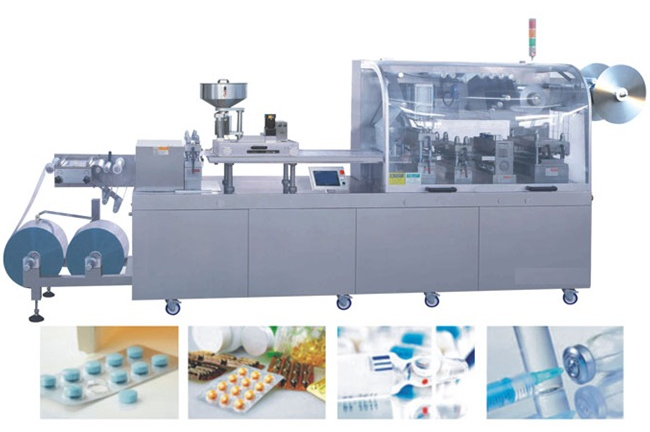
\includegraphics[width=5cm,height=4cm,keepaspectratio]{Datasheets/5Foto.png} 
\\
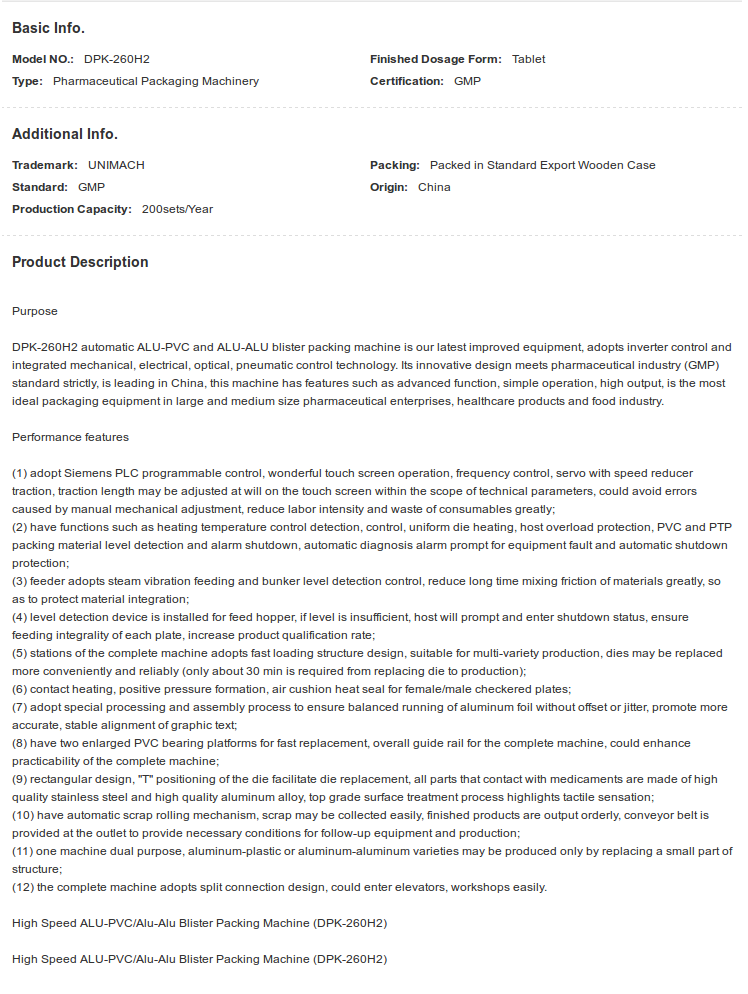
\includegraphics[width=15cm,height=20cm,keepaspectratio]{Datasheets/5MaquinaBlisters.png} 
\newpage

\subsubsection{Máquina de fabricación de cajas}
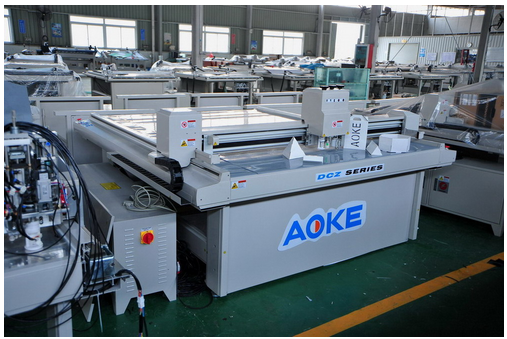
\includegraphics[width=5cm,height=4cm,keepaspectratio]{Datasheets/6Foto.png} 
\\
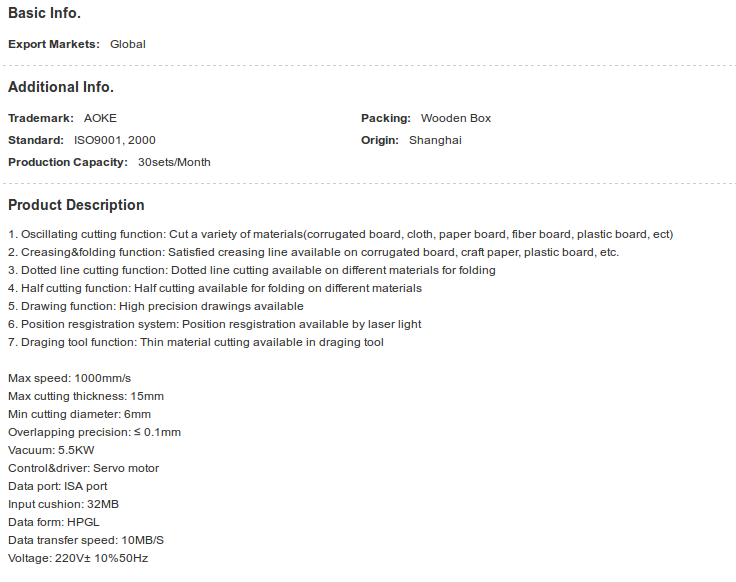
\includegraphics[width=15cm,height=20cm,keepaspectratio]{Datasheets/6MaquinaCajas.png} 
\newpage

\subsubsection{Máquina de empaquetado}
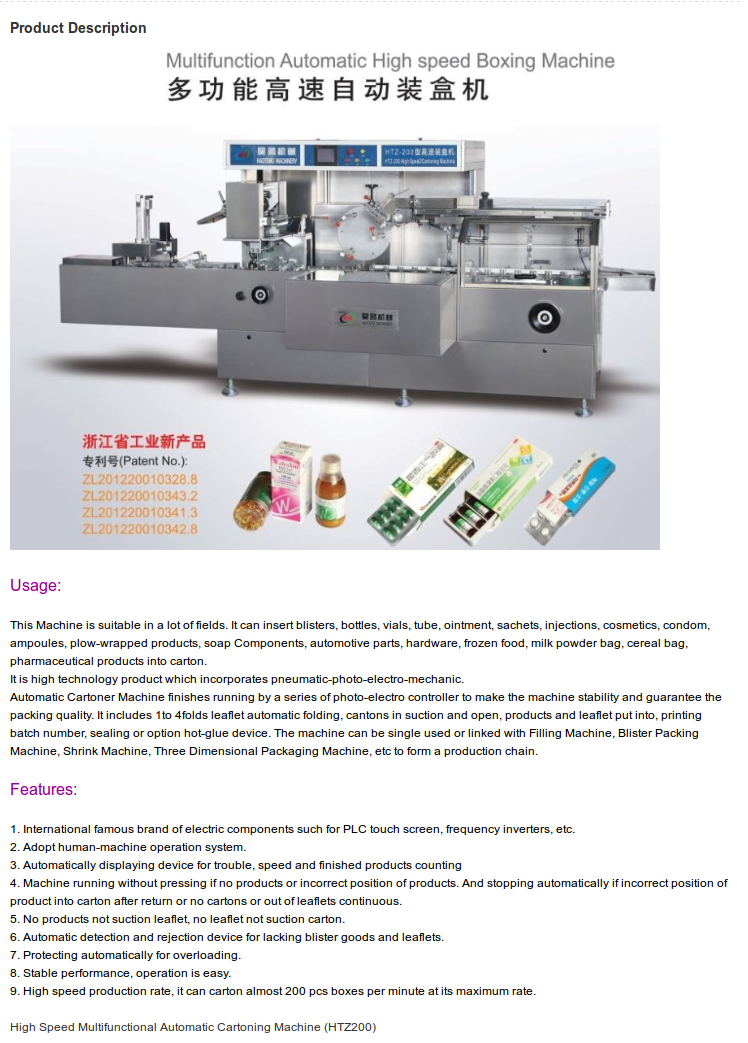
\includegraphics[width=15cm,height=20cm,keepaspectratio]{Datasheets/7MaquinaEmpaquetado.png} 
\newpage
\subsubsection{Robot de paletizado}

\subsection{Planificación}

